\documentclass[12;pt,t]{beamer} % beamer - typ/šablona prezentace

\usepackage[english]{babel}
\usepackage[utf8]{inputenc}
\usepackage[T1]{fontenc}

\usepackage{lmodern}

\usepackage{enumitem} % solve problem with setting bullet character in itemize
% https://stackoverflow.com/a/2823479

\usepackage{graphicx} % inserting images

\usepackage{multicol} % work with multiple columns

\usepackage{xcolor}
\usepackage{listings}


\lstset{basicstyle=\footnotesize\ttfamily,
  showstringspaces=false,
  commentstyle=\color{red},
  keywordstyle=\color{blue},
  escapeinside={(*@}{@*)},
  breaklines=true,
  extendedchars=true,
  inputencoding=utf8
}

\lstdefinelanguage{bettertex}{%
  language     = tex,
  morekeywords = {begin,hline},
}

% nicer source href for images
\definecolor{sourcesclr}{rgb}{.38,.38,.38}
\newcommand{\srctext}[1]{{\fontsize{7}{9}\selectfont\textcolor{sourcesclr}{#1}}}

% Themes: http://www.hartwork.org/beamer-theme-matrix/
\mode<presentation>{\usetheme{Madrid}}
\usecolortheme{beaver}
\beamertemplatenavigationsymbolsempty 
\setbeamertemplate{title page}[default][colsep=0bp,rounded=true]
\setbeamertemplate{itemize items}{-} %$\circ$
\setbeamercolor*{item}{fg=black}
\setbeamertemplate{enumerate item}[default]


\author{Jaroslav Páral}
\institute[paral.jarek@gmail.com]{FI MUNI: PA176\\[0.5cm]}
\title{STM32 programming}


\begin{document}

\frame{\titlepage}

\begin{frame}
\frametitle{Source code}
	\vfill
	\begin{center}
		 \href{https://github.com/JarekParal/FI-MUNI_PA176_STM32-programming}{Github:JarekParal/FI-MUNI\_PA176\_STM32-programming} \\
		 \vfill
		 \url{https://goo.gl/x6BciB}
		 \vfill
		 \href{https://github.com/JarekParal/FI-MUNI_PA176_STM32-programming/blob/master/STM32F103C8_encoders_TrueStudio/Src/main.c}{STM32F103C8\_encoders\_TrueStudio/Src/main.c}
	\end{center}
	
\end{frame}


\begin{frame}
\frametitle{STM32 ARM family}
	\begin{figure}[H]
		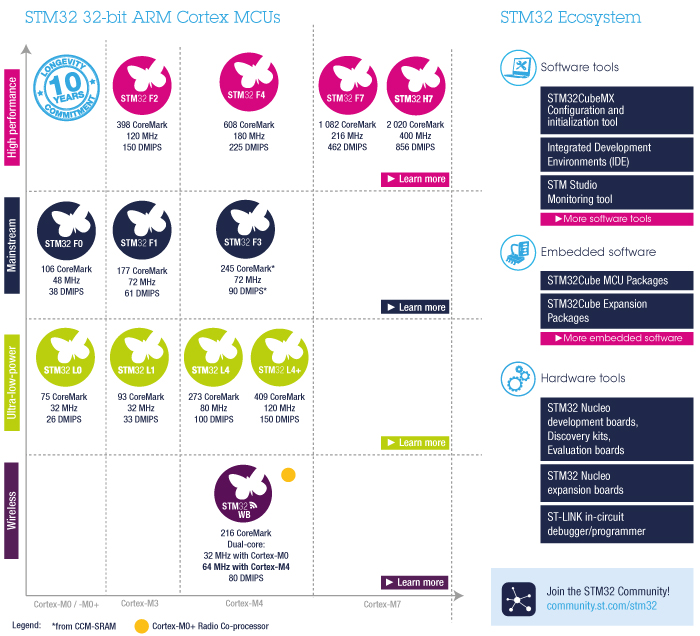
\includegraphics[width=0.6\textwidth]{img/stm32_cl1734.jpg}
		%\caption{STM32 32-bit ARM Cortex MCUs}
	\end{figure}
	\srctext{Image source: \url{http://www.st.com/en/microcontrollers/stm32-32-bit-arm-cortex-mcus.html}}
\end{frame}

\begin{frame}
\frametitle{STM32 ARM family}
	\begin{figure}[H]
		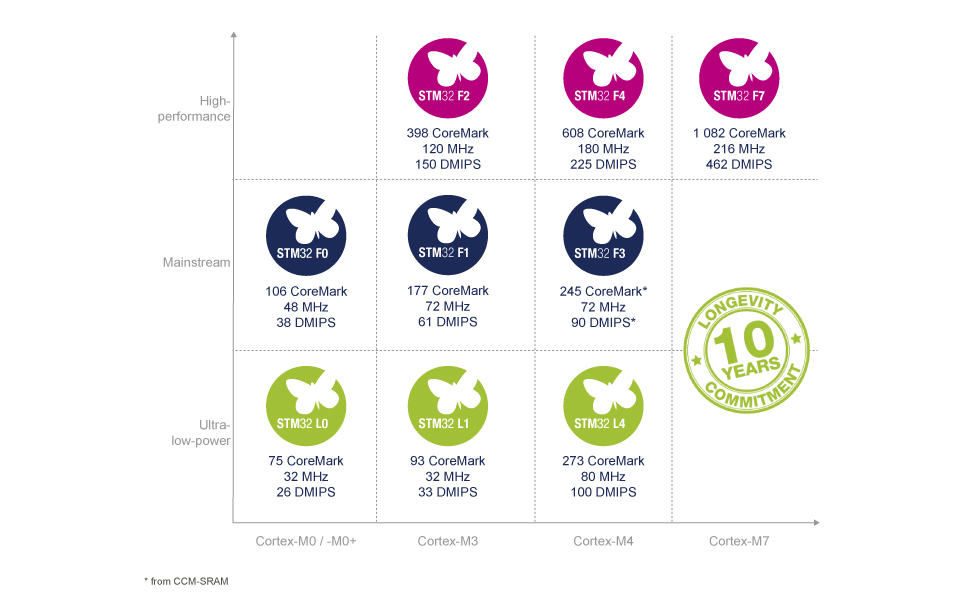
\includegraphics[width=0.9\textwidth]{img/digikey_stm32-cortex.jpg}
	\end{figure}
	\srctext{Image source: \href{https://www.digikey.com/en/product-highlight/s/stmicroelectronics/stm32-overview}{Digikey.com}}
\end{frame}

\begin{frame}
\frametitle{STM32 MCU Nucleo - development board}
	\begin{figure}[H]
		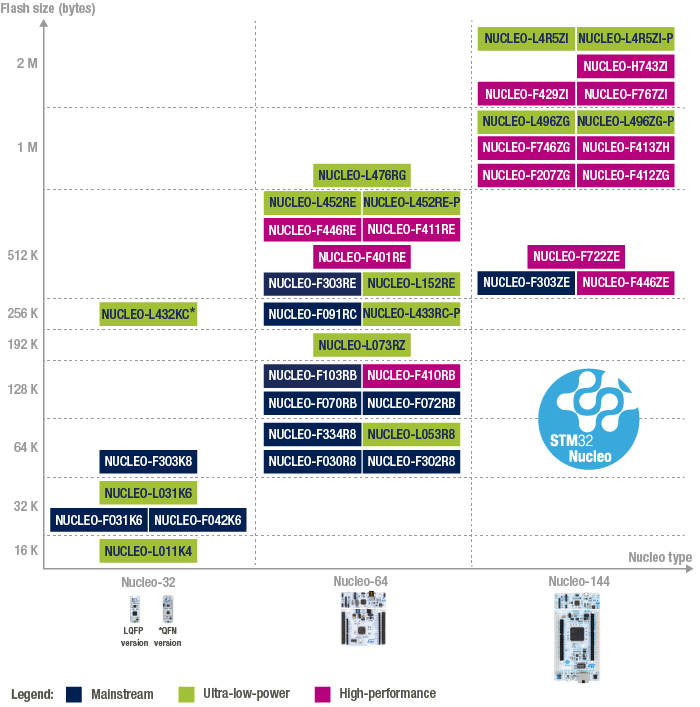
\includegraphics[width=0.6\textwidth]{img/ln1847_stm32_nucleo.jpg}
		%\caption{STM32 Nucleo ecosystem}
	\end{figure}
	\srctext{Image source: \url{http://www.st.com/en/evaluation-tools/stm32-mcu-nucleo.html}}
\end{frame}

\begin{frame}
\frametitle{STM32F1 Series}
	\begin{figure}[H]
		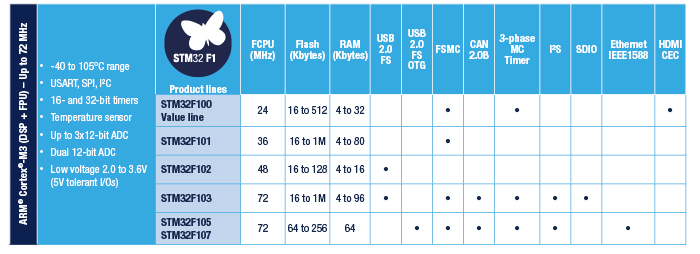
\includegraphics[width=0.9\textwidth]{img/STM32F1_series_SS1031.jpg}
		%\caption{STM32F1 series of mainstream MCUs}
	\end{figure}
	\srctext{Image source: \url{http://www.st.com/en/microcontrollers/stm32f1-series.html}}
\end{frame}

\begin{frame}
\frametitle{STM32F103C8}
	ARM Cortex-M3 MCU with 64 Kbytes Flash, 72 MHz CPU
	\begin{figure}[H]
		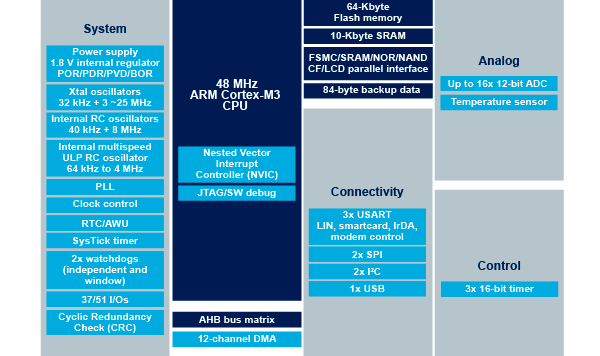
\includegraphics[width=0.8\textwidth]{img/bd_stm32f102x8_64k.jpg}
		%\caption{STM32F103C8}
	\end{figure}
	\srctext{Image source: \url{http://www.st.com/en/microcontrollers/stm32f1-series.html}}
\end{frame}

\begin{frame}
\frametitle{STM32F103C8 - Blue Pill (Ebay / AliExpress - \$2)}
	
	\begin{figure}[H]
		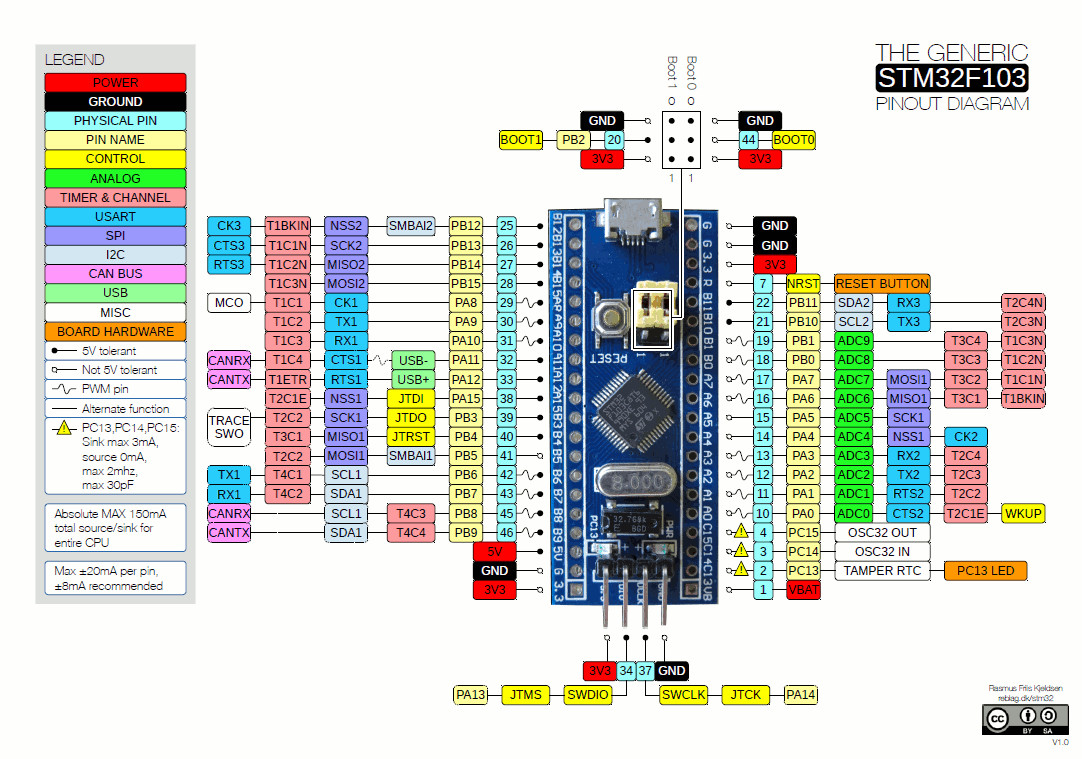
\includegraphics[width=0.8\textwidth]{img/Bluepillpinout.jpg}
		%\caption{STM32F103C8 - Blue Pill}
	\end{figure}
	\srctext{Image source: \url{http://wiki.stm32duino.com/index.php?title=Blue_Pill}}
\end{frame}


\begin{frame}
\frametitle{Tools}
   	IDE (Integrated Development Environment) 
   	\begin{itemize}[label=$\bullet$]
   		\item \href{https://www.iar.com/iar-embedded-workbench/}{IAR-EWARM - just 30-day time-limited evaluation}
   		\item \href{http://www2.keil.com/mdk5/selector}{Keil MDK-Arm Lite - code size limit: 32 KBytes}
   		\item \href{http://www2.keil.com/mdk5/selector}{SW4STM32 - free, without restriction, not too powerful}
   		\item \href{http://www.st.com/en/development-tools/sw4stm32.html}{Attolic TrueSTUDIO}
   		\begin{itemize}[label=$\cdot$]
   			\item free without any restriction
   			\item \href{https://atollic.com/truestudio/}{now own by ST (2017-12-12)}
   			\item similar powerful IDE as IAR or Keil 
   			\item Windows / Linux
   			\item I recommend 
   		\end{itemize} 
   	\end{itemize}
   Other tools
   \begin{itemize}
   	\item \href{https://www.mbed.com/}{Arm Mbed - IoT Device Platform}
   	\item \href{http://www.st.com/en/development-tools/stm32-ides.html}{more info STM32 IDEs}
   \end{itemize}
\end{frame}

\begin{frame}
\frametitle{Tools}  
   	\href{http://www.st.com/en/development-tools/stm32cubemx.html}{STM32CubeMX - initialization code generator}
	\begin{figure}[H]
   		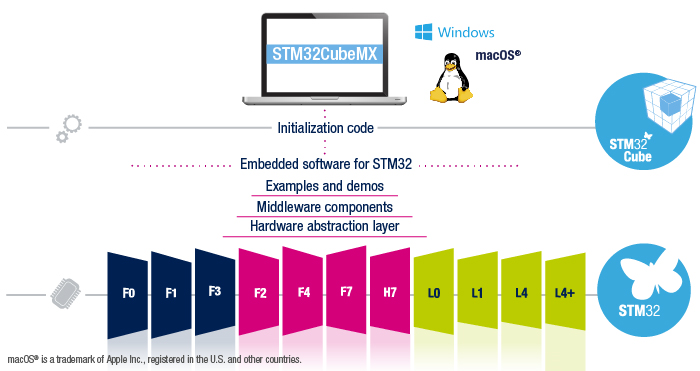
\includegraphics[width=0.9\textwidth]{img/STM32Cube_line_LN1897.jpg}
   		%\caption{STM32F1 series of mainstream MCUs}
   	\end{figure}
   	\srctext{Image source: \url{http://www.st.com/en/embedded-software/stm32cube-mcu-packages.html}}
\end{frame}

\begin{frame}
\frametitle{Libraries and drivers}
	\href{http://www.st.com/en/development-tools/stsw-stm32102.html}{STM32CubeF1 - MCU Package for STM32 F1 series to CubeMX}
	\begin{itemize}[label=$\bullet$]
		\item HAL
		\item Low-Layer APIs 
		\item CMSIS (CORE, DSP, RTOS)
		\item USB
		\item TCP/IP
		\item File system
		\item RTOS
		\item examples for Discovery kits and Evaluation boards
	\end{itemize}		\href{http://www.st.com/en/development-tools/stsw-stm32102.html}{STSW-STM32102 - STM32 Virtual COM Port Driver} \\
\end{frame}

\begin{frame}
\frametitle{Programmer and debugger - ST-Link (AliExpress - \$2)}
	\begin{figure}[H]
		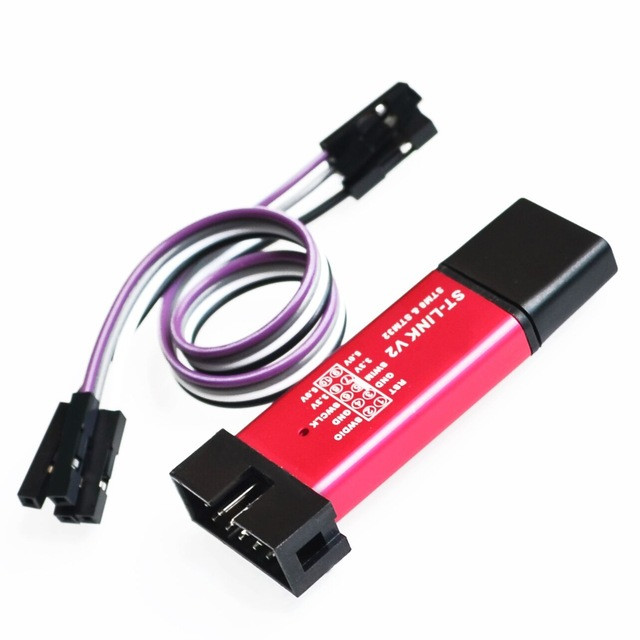
\includegraphics[width=0.55\textwidth]{img/Honeyview_ST-Link-V2.jpg}
		%\caption{ST-Link}
	\end{figure}
	\srctext{Image source: \url{https://goo.gl/kfhSuU/}}
\end{frame}


\begin{frame}[fragile]
	\begin{center}
	\vfill
		How continue? \\
		
		\href{http://www.st.com/en/evaluation-tools/stm32-mcu-nucleo.html?querycriteria=productId=LN1847}{Nucleo board} + \href{http://www.st.com/content/st_com/en/support/learning/stm32-education.html}{STM32 Education} 
		\\
		
		{\tiny 
		\href{http://www.st.com/content/st_com/en/products/evaluation-tools/product-evaluation-tools/mcu-eval-tools/stm32-mcu-eval-tools/stm32-mcu-nucleo/nucleo-l432kc.html}{NUCLEO-L432KC (Arduino Nano compatible)}
	}
	\vfill
	    {\huge Thanks for attention}
	\end{center}
	\vfill
\end{frame}


\end{document}

